\chapter{Mapping. Spheroidal coordinates}

We have seen at the end of the previous chapter that we can work with 2D problems combining {\tt diff\_gl} and
{\tt diff\_leg} objects. This is exactly the purpose of the {\tt mapping} class, that contains all the elements
to work with spherical, and more important, with deformed spheroidal domains. 

\section{Introduction}

Rotating stars are not spherical. The centrifugal force will flatten the star, and this flattening will
be more important as the rotation velocity increases. For this reason, we have to find an appropriate way
to deal with the discretization of the stellar variables in a deformed spheroidal domain.

Note that the problems in which we are interested will involve only axisymmetric quantities, thus essentially 
2D. For that reason, we will restrict the discussion to axisymmetric 2D problems in a spherical-like domain,
but it could be also generalized to other geometries.

\subsection{Coordinate mapping}

We will consider spherical coordinates ($r,\theta,\varphi$). Let $\mathcal{D}$ be an axisymmetric domain centered
in the origin of coordinates ($r=0$) and whose outer boundary $\partial\mathcal{D}$
can be represented by a function $R(\theta)$ that
depends only on the colatitude. We define a new set of coordinates ($\zeta,\theta',\varphi'$) such that 
the new radial-like coordinate $\zeta$ is constant over $\partial\mathcal{D}$. This new spheroidal
coordinates are defined by the transformation:

\begin{equation}
\left\{
\begin{array}{l}
r=r(\zeta,\theta')\\
\theta=\theta'\\
\varphi=\varphi'
\end{array}
\right.
\end{equation}

The problem reduces to find a suitable form for the function $r(\zeta,\theta)$.

In our case we are going a little bit further. We will split the domain $\mathcal{D}$ in $n$ subdomains 
$\mathcal{D}_i$ with $i=0,\ldots,n-1$. The frontiers between this subdomains are represented by a series
of functions $R_i(\theta)$, $i=0,\ldots,n$, such that the $\mathcal{D}_i\in[R_{i}(\theta),R_{i+1}(\theta)]$.
Note that $R_n(\theta)=R(\theta)$ is the outer boundary of the whole domain and, if the domain contains
the origin of coordinates $R_0(\theta)=0$.

We will have also an external domain $\mathcal{D}_{ex}$ that extends from the outer boundary $R_n(\theta)$
to infinity. It will be useful for writing boundary conditions for certain variables as, for example, the
gravitational potential.

\begin{figure}
\centering
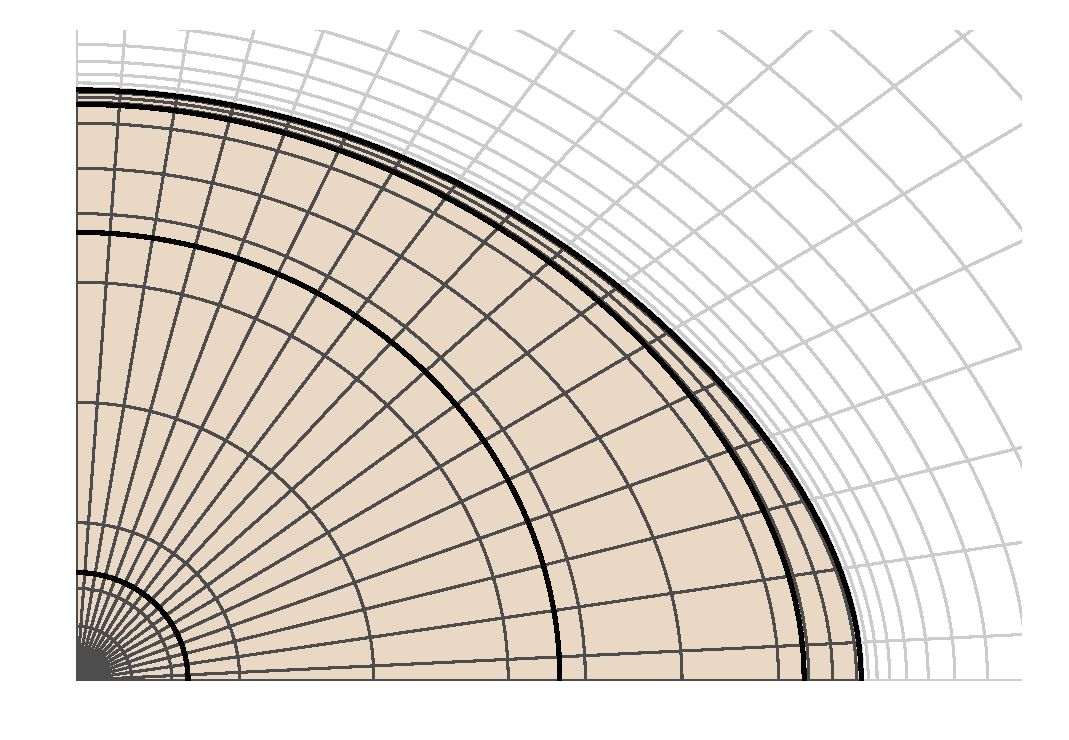
\includegraphics[width=0.8\textwidth]{fig/mapping.eps}
\caption{Coordinate mapping.}
\end{figure}


We will use a technique adopted from \citet{Bonazzola}, in each subdomain $\mathcal{D}_i$ we use a mapping
in the form
\begin{equation}
\label{eq:map}
r(\zeta,\theta)=a_i\xi\Delta\eta_i+R_i(\theta)+A_i(\xi)(\Delta R_i(\theta)-a_i\Delta\eta_i) 
\qquad \mbox{for $\zeta\in[\eta_i,\eta_{i+1}]$}
\end{equation}
where we have defined:
\begin{eqnarray*}
\eta_i&=&R_i(\theta=0)\\
\Delta\eta_i&=&\eta_{i+1}-\eta_i\\
\Delta R_i(\theta)&=&R_{i+1}(\theta)-R_{i}(\theta)\\
\xi&=&\displaystyle\frac{\zeta-\eta_i}{\Delta\eta_i}
\end{eqnarray*} 

The function(s) $A_i(\xi)$ and the constant(s) $a_i$ will determine the final form of the mapping. In particular,
the function $A_i(\xi)$ should verify the following conditions:
\begin{eqnarray*}
r(\eta_i,\theta)=R(\theta) &\longrightarrow& A_i(\xi=0)=0\\
r(\eta_{i+1},\theta)=R_{i+1}(\theta) &\longrightarrow& A_i(\xi=1)=1
\end{eqnarray*}

The simplest possibility is what we will call a linear mapping
\begin{equation}
A_i(\xi)=\xi \qquad a_i=0
\end{equation}
that gives
\begin{equation}
\label{eq:map_linear}
r(\zeta,\theta)=R_i(\theta)+\xi\Delta R_i(\theta)
\end{equation}

In \citet{Bonazzola}, the mapping proposed by the authors satisfies some extra conditions to make it suitable
for spectral methods. For that reason they set $A_i'(\xi=0)=0$ and $A_i'(\xi=1)=0$. Doing
this, the first derivative of the mapping
\begin{equation}
r_\zeta=\frac{\partial r}{\partial\zeta}=a_i+A_i'(\xi)\left(\frac{\Delta R_i(\theta)}{\Delta\eta_i}-a_i\right)
\end{equation}
is constant over the boundaries of the domains. This facilitates the writing of interface conditions for
the derivatives of the variables in the problem when they are expressed in terms of their spectral coefficients.
In this case, we will set
\begin{eqnarray}
\label{eq:map_bonazzola}
A_i(\xi)=-2\xi^3+3\xi^2 &\qquad& \mbox{for $i=1,\ldots,n-1$}\\
A_0(\xi)=-1.5\xi^5+2.5\xi^3&&
\end{eqnarray}
The constant $a_i$ deserves some special attention. We want $r_\zeta>0$, that is, $r$ being monotonically 
increasing with $\zeta$, then $a_i$ should satisfy the condition
\begin{equation}
a_i(A_i'(\xi)-1)<A_i'(\xi)\frac{\Delta R_i(\theta)}{\Delta\eta_i}
\end{equation}
For $A_i'(\xi)=0$ (the boundaries), the condition states $a_i>0$.
When $A'(\xi)<1$, the condition is automatically satisfied (note that $A_i'(\xi)$ is always positive).
But, as $A(\xi)$ should go from 0 at $\xi=0$ to 1 at $\xi=1$, we know that $\max(A_i'(\xi))\ge1$, where the
equality corresponds to the linear mapping that we have seen before. So, in the worst case, the condition
becomes
\begin{equation}
a_i<\frac{1}{1-1/\max(A_i'(\xi))}\frac{\min(\Delta R_i(\theta))}{\Delta\eta_i}
\end{equation}
or, using (\ref{eq:map_bonazzola})
\begin{equation}
\begin{array}{l}
\displaystyle a_i<3\frac{\min(\Delta R_i(\theta))}{\Delta\eta_i} \qquad \mbox{for $i=1,\ldots,n-1$}\\
\displaystyle a_0<\frac{15}{7}\frac{\min(\Delta R_0(\theta))}{\Delta\eta_0}
\end{array}
\end{equation}
In practice, we will take $a_i=1$. This is motivated by the fact that we will work with oblate domains, and
the flattening will increase for the successive subdomains, then $\min(\Delta R_i(\theta))=\Delta\eta_i$,
and the conditions are fully satisfied. Also, working with a fixed value of $a_i$ makes easier to work
with problems where the frontiers between the subdomains are not known a priori, and the jacobian of 
the mapping becomes a smooth function suitable for iterative methods.

The general form of the jacobian of the mapping is defined by the expression
\begin{equation}
\delta r^{i}=J_0^{(i)}(\zeta,\theta)\delta\eta_i+J_1^{(i)}(\zeta,\theta)\delta\Delta\eta_i
+J_2^{(i)}(\zeta,\theta)\delta R_i(\theta)+J_3^{(i)}(\zeta,\theta)\delta\Delta R_i(\theta)
\end{equation}
and using (\ref{eq:map}), for fixed $a_i$
\begin{equation}
\begin{array}{l}
J_0^{(i)}=0\\
J_1^{(i)}=a_i(\xi-A_i(\xi))\\
J_2^{(i)}=1\\
J_3^{(i)}=A_i(\xi)
\end{array}
\end{equation}

For the external domain, we will take 
\begin{equation}
\xi_{ex}=\frac{\zeta-\eta_n}{\eta_n} \qquad \xi\in[0,\infty)
\end{equation}
and
\begin{equation}
r_{ex}(\zeta,\theta)=\xi+R(\theta)
\end{equation}
with jacobian
\begin{equation}
\begin{array}{l}
J_0^{(ex)}=0\\
J_1^{(ex)}=0\\
J_2^{(ex)}=1\\
J_3^{(ex)}=0
\end{array}
\end{equation}


